%%%%%%%%%%%%%%%%%%%%%%%%%%%%%%%%%%%%%%
% LaTeX poster template
% Created by Nathaniel Johnston
% August 2009
% http://www.nathanieljohnston.com/2009/08/latex-poster-template/
%%%%%%%%%%%%%%%%%%%%%%%%%%%%%%%%%%%%%%

\documentclass[final]{beamer}
\usepackage[scale=1.24]{beamerposter}
\usepackage{graphicx}			% allows us to import images

%-----------------------------------------------------------
% Define the column width and poster size
% To set effective sepwid, onecolwid and twocolwid values, first choose how many columns you want and how much separation you want between columns
% The separation I chose is 0.024 and I want 4 columns
% Then set onecolwid to be (1-(4+1)*0.024)/4 = 0.22
% Set twocolwid to be 2*onecolwid + sepwid = 0.464
%-----------------------------------------------------------

\newlength{\sepwid}
\newlength{\onecolwid}
\newlength{\twocolwid}
\newlength{\threecolwid}
\setlength{\paperwidth}{48in}
\setlength{\paperheight}{36in}
\setlength{\sepwid}{0.024\paperwidth}
\setlength{\onecolwid}{0.22\paperwidth}
\setlength{\twocolwid}{0.464\paperwidth}
\setlength{\threecolwid}{0.708\paperwidth}
\setlength{\topmargin}{-0.5in}
\usetheme{confposter}
\usepackage{exscale}

%-----------------------------------------------------------
% The next part fixes a problem with figure numbering. Thanks Nishan!
% When including a figure in your poster, be sure that the commands are typed in the following order:
% \begin{figure}
% \includegraphics[...]{...}
% \caption{...}
% \end{figure}
% That is, put the \caption after the \includegraphics
%-----------------------------------------------------------

\usecaptiontemplate{
\small
\structure{\insertcaptionname~\insertcaptionnumber:}
\insertcaption}

%-----------------------------------------------------------
% Define colours (see beamerthemeconfposter.sty to change these colour definitions)
%-----------------------------------------------------------

\setbeamercolor{block title}{fg=ngreen,bg=white}
\setbeamercolor{block body}{fg=black,bg=white}
\setbeamercolor{block alerted title}{fg=white,bg=dblue!70}
\setbeamercolor{block alerted body}{fg=black,bg=dblue!10}

%-----------------------------------------------------------
% Name and authors of poster/paper/research
%-----------------------------------------------------------

\title{Logical dependencies between classes:\\ how to find them and how to use them ?}
\author{Adelina Diana Stana }
\institute{Department of Computer and Information Technology,  Politehnica University of Timisoara, Romania }

%-----------------------------------------------------------
% Start the poster itself
%-----------------------------------------------------------

\begin{document}
\begin{frame}[t]
  \begin{columns}[t]												% the [t] option aligns the column's content at the top
    \begin{column}{\sepwid}\end{column}			% empty spacer column
    \begin{column}{\onecolwid}
%%%%%%%%%%%%%%%%%%%%%%%%%%%%%%%%%%
\begin{alertblock}{Definition}
       A  \texttt{dependency} is a relationship that shows that an element, or set of elements, requires other elements for their specification or implementation. [ UML Specification]
\end{alertblock}

%%%%%%%%%%%%%%%%%%%%%%%%%%%%%%%%%%
 \begin{block}{Structural dependencies}
      Structural dependencies are the result of source code analysis and can be extracted from : members, call parameters, local variables. 
        \vskip1ex
       \begin{center}
     \begin{figure}
	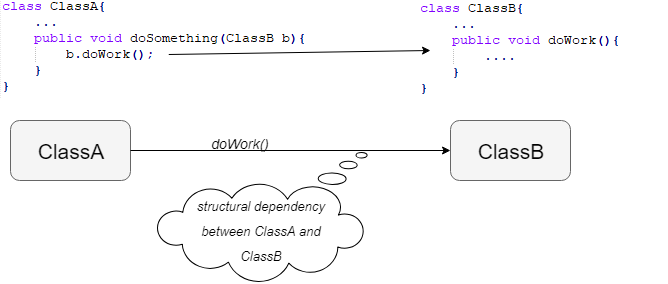
\includegraphics[width=\textwidth]{structural_dep.png}
	\caption{\label{fig:fig}Example of structural dependency between two classes}
     \end{figure}
\end{center}
        \vskip1ex
\end{block}

\vskip2ex
%%%%%%%%%%%%%%%%%%%%%%%%%%%%%%%%%%
\begin{block}{Logical dependencies}
         Logical dependencies are the result of software history analysis and can reveal relationships that are not present in the source code code (structural dependencies).
 
\begin{center}
     \begin{figure}
	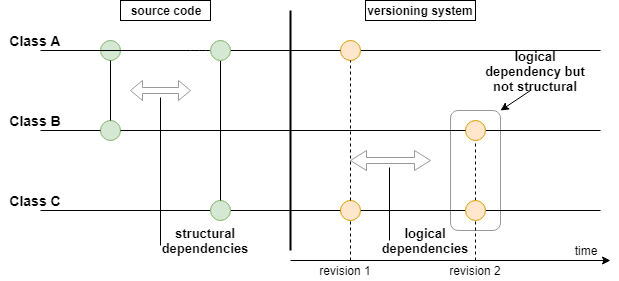
\includegraphics[width=\textwidth]{fig1.png}
	\caption{\label{fig:fig1}Example of logical and structural dependencies}
     \end{figure}
\end{center}

\end{block}
\vskip2ex
\end{column}
%%%%%%%%%%%%%%%%%%%%%%%%%%%%%%%%%%%%%%%%%%%%%%
\begin{column}{\sepwid}\end{column}			
\begin{column}{\threecolwid}					
      \begin{block}{Research questions}
        We build logical dependencies based on three questions :
        \begin{semiverbatim}
 \hskip1ex \textit{\textbf{Question 1:} How the number of files changed in a commit can influence the logical dependencies of the system?}

 \hskip1ex \textit{\textbf{Question 2:} Considering comment changes as valid changes can lead to additional logical dependencies ? }

 \hskip1ex \textit{\textbf{Question 3:} One occurrence of a logical dependency is enough to consider it as valid ?}
        \end{semiverbatim}
\end{block}
%%%%%%%%%%%%%%%%%%%%%%%%%%%%%%%%%%%%%%%%%%%%%%%

\begin{columns}[t,totalwidth=\threecolwid]	% split up that three-column-wide column
        \begin{column}{\onecolwid}
          \begin{block}{Tool for measuring software dependencies}
           In order to answer these research questions, we have built a tool that extracts structural and logical dependencies.
\begin{center}
     \begin{figure}
	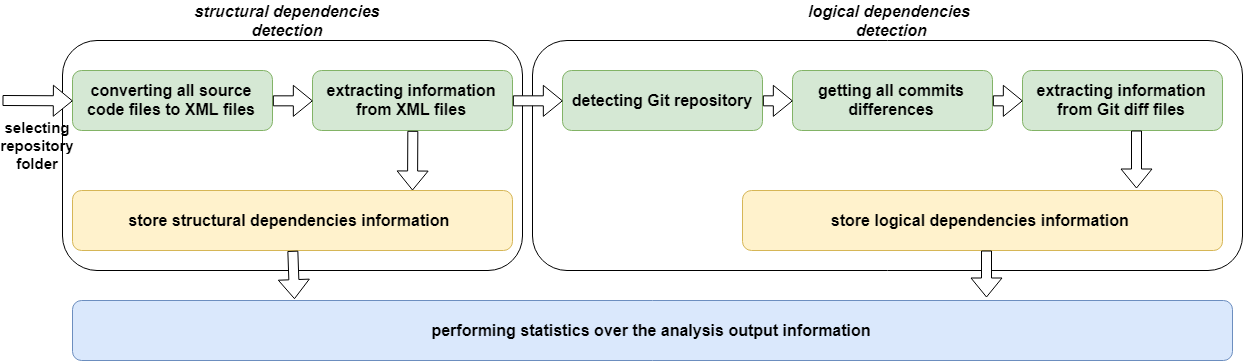
\includegraphics[width=\textwidth]{fig3.png}
	\caption{\label{fig:fig3}Workflow diagram of the tool}
     \end{figure}
\end{center}
The workflow can be delimited by three major steps as it follows:
\begin{semiverbatim}
	\hskip1ex Extracting structural dependencies.

	\hskip1ex  Extracting logical dependencies.

	\hskip1ex  Processing the information extracted.
\end{semiverbatim}
\end{block}
%%%%%%%%%%%%%%%%%%%%%%%%%%%%%%%%%%%%%%%%%%
\vskip3ex
          \setbeamercolor{block alerted title}{fg=black,bg=norange}	% frame color
          \setbeamercolor{block alerted body}{fg=black,bg=white}		% body color
          \begin{alertblock}{Experimental conditions}
           For each system, we extracted its structural dependencies, its logical dependencies and determined the overlap between the two dependencies sets, in various experimental conditions:
            \begin{semiverbatim}
              {\color{blue} -  code comments}

              {\color{blue} - size of commit}

	   {\color{blue} - number of LD occurrences}

            \end{semiverbatim}
          \end{alertblock}    
\end{column}
%%%%%%%%%%%%%%%%%%%%%%%%%%%%%%%%%%%%%%%%%
\begin{column}{\twocolwid}
\begin{block}{Experimental results}
       
\begin{figure}
\centering
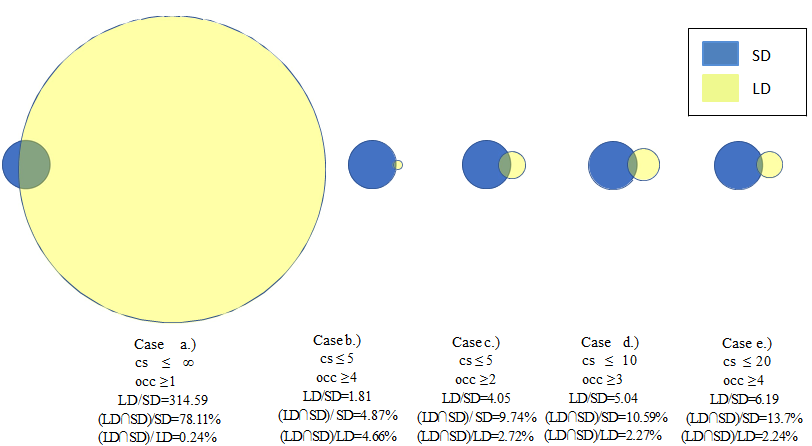
\includegraphics[width=16in]{figvennpdf.png}
\caption{Intersections of logical and structural dependencies, in different cases defined by different combinations of filtering thresholds. }
\end{figure}

\end{block}

    
%%%%%%%%%%%%%%%%%%%%%%%%%%%%%%%%%%%%%%%%

\begin{block}{Conclusions and Future work}
\begin{itemize}
      \item  Large number of structural dependencies are not doubled by logical - systems partially stable
      \item  + -3\% for comments as a change
      \item The number of changed files taken into consideration influence the results
	\begin{itemize}   
	\item big threshold  - not so relevant logical dependencies
	\item small threshold (5~10)  -  more accurate results
    	\end{itemize}
      \item Filtering the logical dependencies after occurrences is good only for projects with a significant number of commits. 
\end{itemize}
Investigate the cause for the large number of logical dependencies which are not overlapping with structural dependencies.
	\end{block}
        \end{column}
      \end{columns}
      \vskip2.5ex
    \end{column}
  \begin{column}{\sepwid}\end{column}			% empty spacer column
 \end{columns}
\end{frame}
\end{document}
